\documentclass{standalone}
\usepackage{tikz}
\usetikzlibrary{patterns, positioning}

\begin{document}
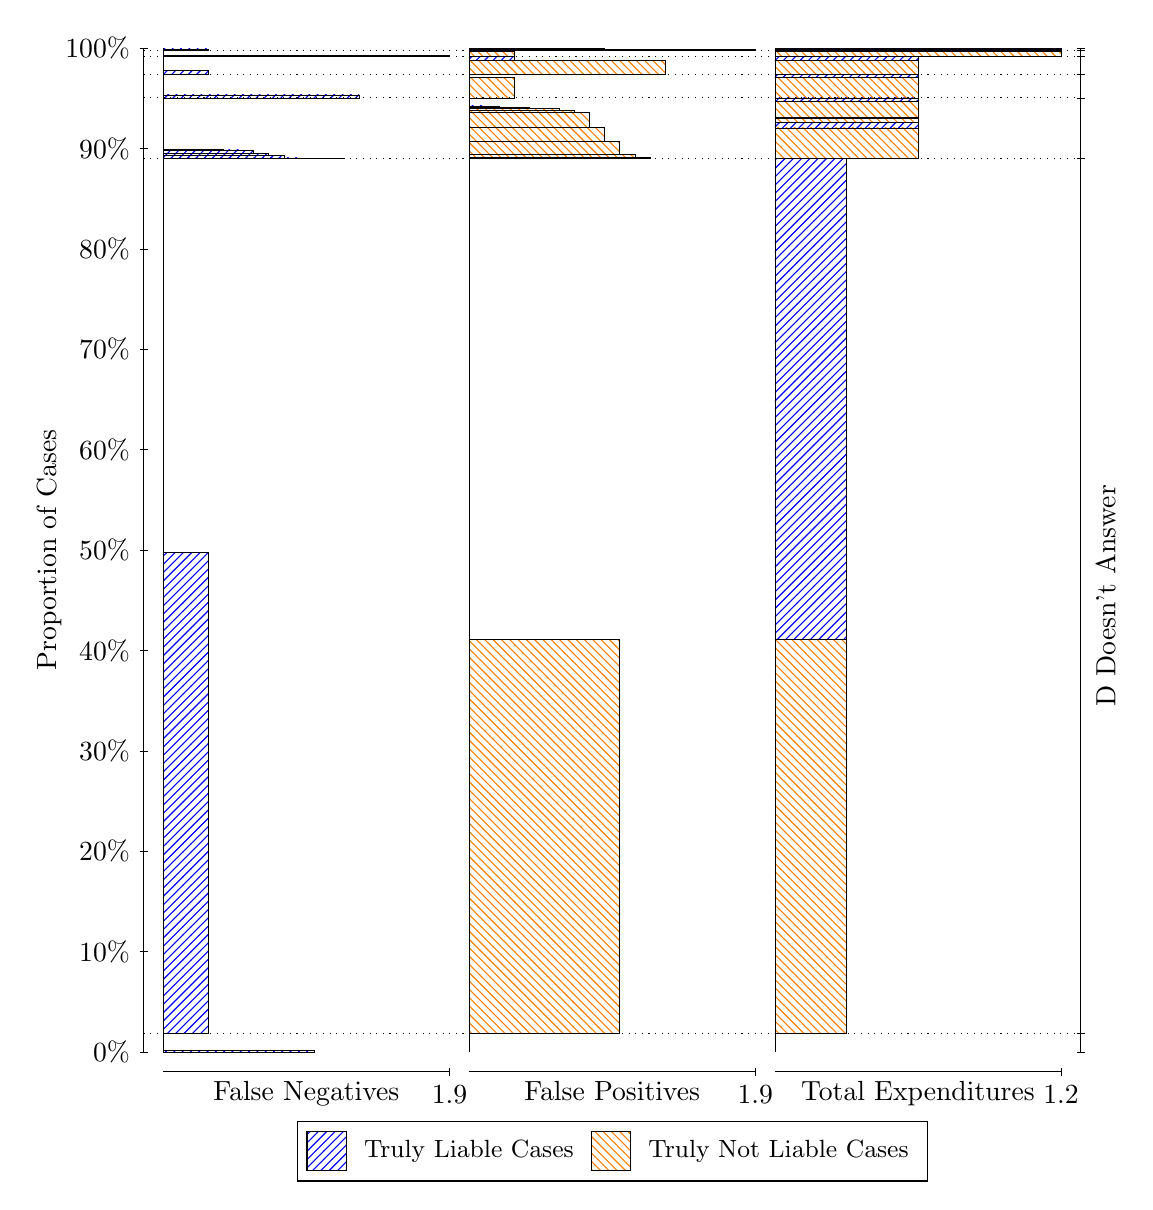
\begin{tikzpicture}
\draw[black, very thin] (1.5,1.75) -- (1.5,14.5);
\node[rotate=90, anchor=center] at (0.3, 8.125) {Proportion of Cases};
\draw[black, very thin] (1.45,1.75) -- (1.55,1.75);
\node[anchor=east] at (1.45, 1.75) {0\%};
\draw[black, very thin] (1.45,3.025) -- (1.55,3.025);
\node[anchor=east] at (1.45, 3.025) {10\%};
\draw[black, very thin] (1.45,4.3) -- (1.55,4.3);
\node[anchor=east] at (1.45, 4.3) {20\%};
\draw[black, very thin] (1.45,5.575) -- (1.55,5.575);
\node[anchor=east] at (1.45, 5.575) {30\%};
\draw[black, very thin] (1.45,6.85) -- (1.55,6.85);
\node[anchor=east] at (1.45, 6.85) {40\%};
\draw[black, very thin] (1.45,8.125) -- (1.55,8.125);
\node[anchor=east] at (1.45, 8.125) {50\%};
\draw[black, very thin] (1.45,9.4) -- (1.55,9.4);
\node[anchor=east] at (1.45, 9.4) {60\%};
\draw[black, very thin] (1.45,10.675) -- (1.55,10.675);
\node[anchor=east] at (1.45, 10.675) {70\%};
\draw[black, very thin] (1.45,11.95) -- (1.55,11.95);
\node[anchor=east] at (1.45, 11.95) {80\%};
\draw[black, very thin] (1.45,13.225) -- (1.55,13.225);
\node[anchor=east] at (1.45, 13.225) {90\%};
\draw[black, very thin] (1.45,14.5) -- (1.55,14.5);
\node[anchor=east] at (1.45, 14.5) {100\%};

\draw[black, very thin] (13.4,1.75) -- (13.4,14.5);
\draw[black, very thin] (13.35,1.75) -- (13.45,1.75);
\node[anchor=west] at (13.35, 1.75) {};
\draw[black, very thin] (13.35,1.9888) -- (13.45,1.9888);
\node[anchor=west] at (13.35, 1.9888) {};
\draw[black, very thin] (13.35,13.094) -- (13.45,13.094);
\node[anchor=west] at (13.35, 13.094) {};
\draw[black, very thin] (13.35,13.868) -- (13.45,13.868);
\node[anchor=west] at (13.35, 13.868) {};
\draw[black, very thin] (13.35,14.165) -- (13.45,14.165);
\node[anchor=west] at (13.35, 14.165) {};
\draw[black, very thin] (13.35,14.396) -- (13.45,14.396);
\node[anchor=west] at (13.35, 14.396) {};
\draw[black, very thin] (13.35,14.471) -- (13.45,14.471);
\node[anchor=west] at (13.35, 14.471) {};
\draw[black, very thin] (13.35,14.5) -- (13.45,14.5);
\node[anchor=west] at (13.35, 14.5) {};

\draw[black, very thin, pattern color=blue, pattern=north east lines] (1.75,1.75) rectangle (3.6623,1.7751);
\draw[black, very thin, pattern color=orange, pattern=north west lines] (1.75,1.7751) rectangle (1.75,1.9888);
\draw[black, very thin, pattern color=blue, pattern=north east lines] (1.75,1.9888) rectangle (2.3237,8.095);
\draw[black, very thin, pattern color=orange, pattern=north west lines] (1.75,8.095) rectangle (1.75,13.094);
\draw[black, very thin, pattern color=blue, pattern=north east lines] (1.75,13.094) rectangle (4.0447,13.095);
\draw[black, very thin, pattern color=blue, pattern=north east lines] (1.75,13.095) rectangle (3.8535,13.097);
\draw[black, very thin, pattern color=blue, pattern=north east lines] (1.75,13.097) rectangle (3.6623,13.101);
\draw[black, very thin, pattern color=blue, pattern=north east lines] (1.75,13.101) rectangle (3.4711,13.103);
\draw[black, very thin, pattern color=blue, pattern=north east lines] (1.75,13.103) rectangle (3.4711,13.106);
\draw[black, very thin, pattern color=blue, pattern=north east lines] (1.75,13.106) rectangle (3.2798,13.138);
\draw[black, very thin, pattern color=blue, pattern=north east lines] (1.75,13.138) rectangle (3.0886,13.165);
\draw[black, very thin, pattern color=blue, pattern=north east lines] (1.75,13.165) rectangle (2.8974,13.196);
\draw[black, very thin, pattern color=blue, pattern=north east lines] (1.75,13.196) rectangle (2.7061,13.206);
\draw[black, very thin, pattern color=blue, pattern=north east lines] (1.75,13.206) rectangle (2.5149,13.216);
\draw[black, very thin, pattern color=orange, pattern=north west lines] (1.75,13.216) rectangle (1.75,13.868);
\draw[black, very thin, pattern color=blue, pattern=north east lines] (1.75,13.868) rectangle (4.236,13.905);
\draw[black, very thin, pattern color=orange, pattern=north west lines] (1.75,13.905) rectangle (1.75,14.165);
\draw[black, very thin, pattern color=blue, pattern=north east lines] (1.75,14.165) rectangle (2.3237,14.219);
\draw[black, very thin, pattern color=orange, pattern=north west lines] (1.75,14.219) rectangle (1.75,14.396);
\draw[black, very thin, pattern color=blue, pattern=north east lines] (1.75,14.396) rectangle (5.3833,14.408);
\draw[black, very thin, pattern color=orange, pattern=north west lines] (1.75,14.408) rectangle (1.75,14.471);
\draw[black, very thin, pattern color=blue, pattern=north east lines] (1.75,14.471) rectangle (2.3237,14.488);
\draw[black, very thin, pattern color=orange, pattern=north west lines] (1.75,14.488) rectangle (1.75,14.5);
\draw[black, very thin, pattern color=orange, pattern=north west lines] (5.6333,1.75) rectangle (5.6333,1.9637);
\draw[black, very thin, pattern color=blue, pattern=north east lines] (5.6333,1.9637) rectangle (5.6333,1.9888);
\draw[black, very thin, pattern color=orange, pattern=north west lines] (5.6333,1.9888) rectangle (7.5456,6.9873);
\draw[black, very thin, pattern color=blue, pattern=north east lines] (5.6333,6.9873) rectangle (5.6333,13.094);
\draw[black, very thin, pattern color=orange, pattern=north west lines] (5.6333,13.094) rectangle (7.9281,13.113);
\draw[black, very thin, pattern color=orange, pattern=north west lines] (5.6333,13.113) rectangle (7.7368,13.152);
\draw[black, very thin, pattern color=orange, pattern=north west lines] (5.6333,13.152) rectangle (7.5456,13.316);
\draw[black, very thin, pattern color=orange, pattern=north west lines] (5.6333,13.316) rectangle (7.3544,13.491);
\draw[black, very thin, pattern color=orange, pattern=north west lines] (5.6333,13.491) rectangle (7.1632,13.682);
\draw[black, very thin, pattern color=orange, pattern=north west lines] (5.6333,13.682) rectangle (6.9719,13.707);
\draw[black, very thin, pattern color=orange, pattern=north west lines] (5.6333,13.707) rectangle (6.7807,13.729);
\draw[black, very thin, pattern color=orange, pattern=north west lines] (5.6333,13.729) rectangle (6.5895,13.737);
\draw[black, very thin, pattern color=orange, pattern=north west lines] (5.6333,13.737) rectangle (6.3982,13.745);
\draw[black, very thin, pattern color=blue, pattern=north east lines] (5.6333,13.745) rectangle (6.0158,13.755);
\draw[black, very thin, pattern color=blue, pattern=north east lines] (5.6333,13.755) rectangle (5.8246,13.765);
\draw[black, very thin, pattern color=blue, pattern=north east lines] (5.6333,13.765) rectangle (5.6333,13.868);
\draw[black, very thin, pattern color=orange, pattern=north west lines] (5.6333,13.868) rectangle (6.207,14.127);
\draw[black, very thin, pattern color=blue, pattern=north east lines] (5.6333,14.127) rectangle (5.6333,14.165);
\draw[black, very thin, pattern color=orange, pattern=north west lines] (5.6333,14.165) rectangle (8.1193,14.341);
\draw[black, very thin, pattern color=blue, pattern=north east lines] (5.6333,14.341) rectangle (6.207,14.396);
\draw[black, very thin, pattern color=orange, pattern=north west lines] (5.6333,14.396) rectangle (6.207,14.459);
\draw[black, very thin, pattern color=blue, pattern=north east lines] (5.6333,14.459) rectangle (5.6333,14.471);
\draw[black, very thin, pattern color=orange, pattern=north west lines] (5.6333,14.471) rectangle (9.2667,14.483);
\draw[black, very thin, pattern color=blue, pattern=north east lines] (5.6333,14.483) rectangle (7.3544,14.5);
\draw[black, very thin, pattern color=orange, pattern=north west lines] (9.5167,1.75) rectangle (9.5167,1.9637);
\draw[black, very thin, pattern color=blue, pattern=north east lines] (9.5167,1.9637) rectangle (9.5167,1.9888);
\draw[black, very thin, pattern color=orange, pattern=north west lines] (9.5167,1.9888) rectangle (10.425,6.9873);
\draw[black, very thin, pattern color=blue, pattern=north east lines] (9.5167,6.9873) rectangle (10.425,13.094);
\draw[black, very thin, pattern color=orange, pattern=north west lines] (9.5167,13.094) rectangle (11.333,13.487);
\draw[black, very thin, pattern color=blue, pattern=north east lines] (9.5167,13.487) rectangle (11.333,13.56);
\draw[black, very thin, pattern color=orange, pattern=north west lines] (9.5167,13.56) rectangle (11.333,13.611);
\draw[black, very thin, pattern color=blue, pattern=north east lines] (9.5167,13.611) rectangle (11.333,13.621);
\draw[black, very thin, pattern color=orange, pattern=north west lines] (9.5167,13.621) rectangle (11.333,13.829);
\draw[black, very thin, pattern color=blue, pattern=north east lines] (9.5167,13.829) rectangle (11.333,13.868);
\draw[black, very thin, pattern color=orange, pattern=north west lines] (9.5167,13.868) rectangle (11.333,14.127);
\draw[black, very thin, pattern color=blue, pattern=north east lines] (9.5167,14.127) rectangle (11.333,14.165);
\draw[black, very thin, pattern color=orange, pattern=north west lines] (9.5167,14.165) rectangle (11.333,14.341);
\draw[black, very thin, pattern color=blue, pattern=north east lines] (9.5167,14.341) rectangle (11.333,14.396);
\draw[black, very thin, pattern color=orange, pattern=north west lines] (9.5167,14.396) rectangle (13.15,14.459);
\draw[black, very thin, pattern color=blue, pattern=north east lines] (9.5167,14.459) rectangle (13.15,14.471);
\draw[black, very thin, pattern color=orange, pattern=north west lines] (9.5167,14.471) rectangle (13.15,14.483);
\draw[black, very thin, pattern color=blue, pattern=north east lines] (9.5167,14.483) rectangle (13.15,14.5);
\draw[black, dotted] (1.5,1.9888) -- (13.4,1.9888);
\draw[black, dotted] (1.5,13.094) -- (13.4,13.094);
\draw[black, dotted] (1.5,13.868) -- (13.4,13.868);
\draw[black, dotted] (1.5,14.165) -- (13.4,14.165);
\draw[black, dotted] (1.5,14.396) -- (13.4,14.396);
\draw[black, dotted] (1.5,14.471) -- (13.4,14.471);
\draw[black, very thin] (1.75,1.5) -- (5.3833,1.5);
\node[anchor=north] at (3.5667, 1.5) {False Negatives};
\draw[black, very thin] (5.3833,1.45) -- (5.3833,1.55);
\node[anchor=north] at (5.3833, 1.45) {1.9};

\draw[black, very thin] (5.6333,1.5) -- (9.2667,1.5);
\node[anchor=north] at (7.45, 1.5) {False Positives};
\draw[black, very thin] (9.2667,1.45) -- (9.2667,1.55);
\node[anchor=north] at (9.2667, 1.45) {1.9};

\draw[black, very thin] (9.5167,1.5) -- (13.15,1.5);
\node[anchor=north] at (11.333, 1.5) {Total Expenditures};
\draw[black, very thin] (13.15,1.45) -- (13.15,1.55);
\node[anchor=north] at (13.15, 1.45) {1.2};


\node[black, centered, rotate=90] at (13.72, 7.5412) {D Doesn't Answer};






\draw (7.449999999999999,1.5) node[draw=none] (baseCoordinate) {};
\begin{scope}[align=center]
        \matrix[scale=0.5, draw=black, below=0.5cm of baseCoordinate, nodes={draw}, column sep=0.1cm]{
            \node[rectangle, draw, minimum width=0.5cm, minimum height=0.5cm, pattern=north east lines, pattern color=blue] {}; &
            \node[draw=none, font=\small] (B) {Truly Liable Cases}; &
            \node[rectangle, draw, minimum width=0.5cm, minimum height=0.5cm, pattern=north west lines, pattern color=orange] {}; &
            \node[draw=none, font=\small] (B) {Truly Not Liable Cases}; \\
            };
\end{scope}

\end{tikzpicture}
\end{document}